\documentclass[journal]{IEEEtran}
\usepackage[utf8]{inputenc}
\usepackage{amsmath, amssymb, amsfonts}
\usepackage{graphicx}
\usepackage{booktabs}
\usepackage{cite}
\usepackage{subcaption}

\title{Robust Neural-Algorithmic Framework for Directed $t$-Spanner Construction in Metropolitan Road Networks: Integrating Fuzzy-Inference Pruning, Epistemic Uncertainty, and Continual Learning}
\author{Soheyl Falahzade}

\begin{document}
\maketitle

\begin{abstract}
Real-time routing in Intelligent Transportation Systems (ITS) is severely bottlenecked by the $O(m \cdot (n + m \log n))$ computational complexity associated with constructing exact geometric $t$-spanners on large-scale urban topologies. While machine learning has emerged as a promising paradigm to bypass these computational limits, standard neural predictors lack formal topological guarantees and rely on a single hard decision threshold that ignores the structural importance of individual edges. This paper introduces a robust hybrid neural-algorithmic framework that (i) shifts the heavy computational burden of spanner construction to an offline representation learning phase while enforcing strict structural constraints online via a cutoff-bounded directed repair procedure, and (ii) replaces the conventional hard-threshold pruning decision with a Mamdani-style fuzzy inference system that jointly reasons over the network's epistemic uncertainty (via Monte Carlo Dropout) and each edge's structural importance (via Edge Betweenness Centrality). Experimental evaluations across three heterogeneous urban fabrics (Eindhoven, Paris, and Rome), each validated over 15--18 independent stochastic seeds at matched sparsification levels, show that the proposed fuzzy pruning mechanism consistently requires fewer post-hoc geometric repairs than both a genetic-algorithm-tuned deterministic threshold with active self-correcting feedback (7.1--16.6\% fewer repairs) and a sparsity-matched random pruning baseline (0.4--10.2\% fewer repairs), across every tested city without exception. We further report, with full transparency, that a single-parameter threshold search does not by itself benefit from evolutionary optimization over random search under equal evaluation budget -- underscoring that the genuine value of evolutionary search in this framework lies in the higher-dimensional joint optimization of loss weights and calibration parameters, not in scalar threshold tuning. Under extreme network corruption, the uncertainty-aware framework maintains full Strong Connectivity (SCC) and a bounded directed stretch factor across all tested configurations.
\end{abstract}

\begin{IEEEkeywords}
Intelligent Transportation Systems, Graph Neural Networks, $t$-Spanner, Strongly Connected Components, Epistemic Uncertainty, Fuzzy Inference Systems, Continual Learning, Genetic Algorithms, High-Performance Computing.
\end{IEEEkeywords}

\section{Introduction}
Modern navigation engines, dynamic fleet management systems, and cooperative autonomous vehicles rely heavily on spatial graph sparsification to minimize the search space of $A^*$ or Dijkstra-based routing agents. In the domain of computational geometry, a directed $t$-spanner $H = (V, E')$ of a spatial graph $G = (V, E)$ is a sparse subgraph that preserves the shortest path distances between any pair of vertices within a strict multiplicative stretch factor $t$:
\begin{equation}
    d_H(u, v) \le t \cdot d_G(u, v) \quad \forall u, v \in V
\end{equation}

In intelligent transportation systems (ITS), maintaining the topological integrity of directed networks is extremely challenging due to asymmetric edge weights arising from one-way streets, turn restrictions, and dynamic traffic congestion. Traditional routing engines struggle with dynamic overheads. Recent paradigm shifts in intelligent transportation systems emphasize the integration of deep learning estimators for real-time route planning on asymmetric topologies [18], yet enforcing strict geometric bounds remains an unresolved challenge.

Historically, constructing high-quality geometric spanners has relied on the classic Greedy Spanner algorithm, which exhibits a computational complexity of $O(m \cdot (n + m \log n))$ using standard Dijkstra implementations. While theoretically optimal in terms of degree, weight, and edge count, this iterative construction is computationally prohibitive for metropolitan-scale directed networks.

To address this challenge, researchers have recently turned to Graph Neural Networks (GNNs) to predict edge importance and sparsify road networks in a data-driven manner. However, pure deep learning methods suffer from a critical flaw: they lack mathematical guarantees. A GNN may classify a critical highway bridge as ``prunable'' based on its local neighborhood features, resulting in infinite stretch (disconnection) or catastrophic detours. This risk is further amplified when the neural model is exposed to out-of-distribution (OOD) city topologies or noisy spatial data, and is further compounded by the common practice of collapsing the pruning decision to a single hard threshold that discards information about an edge's structural role.

In this paper, we propose a robust, hybrid neural-algorithmic framework, named \textit{Geo-SmartSpanner}, which bridges the gap between statistical learning and hard geometric constraints. Our framework uses a scale-invariant GNN with Monte Carlo Dropout to propose candidate pruning lists with well-calibrated confidence scores, and replaces the conventional hard threshold with a fuzzy inference mechanism that reasons jointly over model confidence and edge centrality. To guarantee the $t$-spanner property, we implement a parallelized, directed, batch-sequential geometric repair module that intercepts pruning decisions only when a theoretical violation is detected.

The key contributions of this paper are summarized as follows:
\begin{itemize}
    \item We present a decoupled neural-algorithmic framework that shifts the complexity of directed $t$-spanner construction from $O(m \cdot (n + m \log n))$ offline to a fast, near-linear online inference and verification pipeline, empirically validated to yield a 5.97--26.19x wall-clock speedup over classic greedy construction across four metropolitan networks.
    \item We introduce an active geometric feedback loop that utilizes the failures of the neural network (repaired edges) to fine-tune the GNN parameters on a per-city basis, creating a self-correcting geometric model.
    \item We propose a directed Bounded-Stretch GLV-Repair algorithm, accelerated via cutoff-bounded Dijkstra search, that maintains 100\% Strongly Connected Components (SCC) and strictly bounds the directed stretch factor below 1.5 under extreme spatial noise.
    \item We integrate a meta-evolutionary optimization layer based on Genetic Algorithms (GA) for the joint, multi-parameter calibration of loss weights and uncertainty coefficients, while transparently reporting that scalar threshold search does not itself benefit from evolutionary search over random search under equal evaluation budget.
    \item We propose a Mamdani-style fuzzy inference mechanism that replaces the hard pruning threshold, jointly reasoning over epistemic uncertainty and structural centrality, and demonstrate -- across 15--18 independent seeds per city -- that it consistently outperforms both the GA-tuned threshold and a sparsity-matched random baseline in every tested city.
\end{itemize}

\section{Related Work}
The study of geometric networks and spanner construction was pioneered by several seminal works. Graph spanners were first introduced by Peleg and Schaffer [1] in the context of distributed computing, and extended to planar structures by Chew [2]. Smid [3] provided a comprehensive analysis of closest-point problems and spanner networks. Farshi and Gudmundsson [6] provided the first extensive experimental evaluation of geometric $t$-spanners, highlighting the trade-offs between different quality measures such as degree, weight, and diameter. Bose et al. [7] subsequently reduced the naive cubic time complexity of the greedy spanner to near-quadratic bounds. However, as demonstrated by Bakhshesh and Farshi [8], even optimized variants like the gap-greedy spanner suffer from substantial computational overhead in practice, requiring several minutes to process small point sets.

The theoretical complexity of spanner design in directed graphs (oriented spanners) was recently explored by Buchin et al. [13], who proved that computing oriented spanners with optimal dilation is NP-Hard on general directed graphs. To address this computational bottleneck in practice, recent literature has shifted towards heuristic approximation. In 2026, Buchin, Rehs, and Scheele [14] introduced the concept of constructing ``doppelgangers'' of greedy geometric spanners, seeking fast algorithms that can mimic the sparseness of the greedy spanner in polynomial time. Recent advancements have expanded fault-tolerant spanner designs to planar structures [12] and proposed greedy strategies for region-fault resilient geometric networks [11], yet their computational cost under real-time directed constraints remains a significant bottleneck.

While machine learning has recently been applied to network sparsification, existing neural graph models are typically transductive and fail to guarantee connectivity. Our work differs from these previous approaches by combining the inductive generalization of Graph Neural Networks with the exact, directed verification of computational geometry, and by replacing the conventional hard pruning threshold with a fuzzy inference mechanism grounded in structural centrality, providing a highly scalable and mathematically robust solution to the directed $t$-spanner problem.

\section{Proposed Methodology}

Our framework consists of several tightly coupled components designed to ensure topological safety and high-performance inference under directed traffic constraints.

\subsection{Uncertainty-Aware Neural Edge Classification}
To classify edges, we implement an inductive \texttt{GeometricEdgeSAGE} architecture, building upon the inductive framework proposed by Hamilton et al. [20]. To ensure generalization across cities with different coordinate systems, we engineer scale- and symmetry-invariant spatial features for each edge $i = (u, v) \in E$:
\begin{equation}
    f_i = \left[ \bar{d}(u,v), deg_{in}(u), deg_{out}(v), \mathcal{C}(u, v) \right]
\end{equation}
where $\bar{d}(u, v)$ is the locally normalized road segment length, $deg$ represents node degrees, and $\mathcal{C}$ denotes the local edge betweenness centrality.

Instead of relying on deterministic predictions, which are vulnerable to noise, we estimate the epistemic uncertainty of our GNN using Monte Carlo (MC) Dropout. During online inference, we perform $M$ stochastic forward passes by keeping the dropout layers active:
\begin{equation}
    \mu(i) = \frac{1}{M} \sum_{j=1}^{M} f_\theta(x_i)_j
\end{equation}
\begin{equation}
    \sigma^2(i) = \frac{1}{M} \sum_{j=1}^{M} \left( f_\theta(x_i)_j - \mu(i) \right)^2
\end{equation}

The calibrated pruning-relevant score is then:
\begin{equation}
    \hat{y}_i = \mu(i) + \lambda \cdot \sigma(i)
\end{equation}
Section~\ref{sec:fuzzy} describes how $\hat{y}_i$ is combined with structural centrality via fuzzy inference to reach the final pruning decision, replacing a single hard threshold on $\hat{y}_i$ alone.

\subsection{Topological Safeguards \& Directed GLV-Repair}
To prevent catastrophic structural disconnections, we first apply a hard topological lock. Let $E_{lock}$ be the set of edges incident to low-degree boundary vertices:
\begin{equation}
    E_{lock} = \{ (u, v) \in E \mid deg_{in}(v) \le 1 \lor deg_{out}(u) \le 1 \}
\end{equation}
These edges are strictly protected and never pruned, preserving the basic connectivity of peripheral neighborhoods.

The remaining candidate edges in $E_{prune} \setminus E_{lock}$ are processed using a \textit{Batch-Sequential GLV-Repair} algorithm. In undirected graphs, pruning decisions can be made independently. However, in directed graphs, pruning can cause asymmetric routing bottlenecks, a phenomenon we refer to as the \textit{Blind Batch-Pruning Paradox}.

To resolve this paradox, we sort $E_{prune}$ by edge length and divide it into batches of size $B = 250$. For each batch, we evaluate the shortest path on the remaining sparse graph $H$ using parallelized, directed Dijkstra search. For each pruned edge $e = (u, v) \in E_{prune}$, we check:
\begin{equation}
    d_H(u, v) \le t \cdot w(e)
\end{equation}
where $t = 1.5$ is the target stretch limit. If this condition is violated, $e$ is restored to $H$. Because we process in batches, any restored edge in batch $k$ immediately serves as a valid detour for subsequent batches, preventing redundant edge restorations.

\subsection{Meta-Evolutionary Threshold Selection}
To avoid arbitrary thresholding and systematic biases, we deploy a Genetic Algorithm (GA) to jointly search for Pareto-optimal values of $\lambda$, $\tau$, and the loss weights $w_1, w_2$, navigating the non-convex multi-objective landscape defined by:
\begin{equation}
    \text{Fitness} = w_1 \cdot \text{Sparsification} - w_2 \cdot \max_{u,v} \left( \frac{d_H(u,v)}{d_G(u,v)} - t \right)
\end{equation}
We note that this joint, multi-parameter search is where the genetic algorithm demonstrates genuine value; Section~\ref{sec:ga-vs-rs} reports a controlled experiment showing that for the restricted single-parameter (scalar threshold) sub-problem, a genetic algorithm offers no measurable advantage over random search under equal evaluation budget -- a finding we report transparently rather than omit.

\subsection{Fuzzy-Inference Pruning Decision}
\label{sec:fuzzy}

A hard decision threshold on the calibrated score $\hat{y}_i$ (Eq. 5) treats all edges near the decision boundary identically, regardless of their structural role in the network. To address this, we replace the hard threshold with a Mamdani-style fuzzy inference system that combines two normalized inputs per edge $i$: the calibrated score $\hat{y}_i \in [0,1]$ and the edge betweenness centrality $C(u,v) \in [0,1]$ (min-max normalized per city).

Each input is partitioned into three linguistic terms (\textit{Low}, \textit{Medium}, \textit{High}) using triangular membership functions:
\begin{equation}
    \mu_{\text{Low}}(x) = \max\left(0, \min\left(\frac{x - a_1}{b_1 - a_1}, \frac{c_1 - x}{c_1 - b_1}\right)\right)
\end{equation}
with analogous definitions for $\mu_{\text{Medium}}$ and $\mu_{\text{High}}$, parameterized by knot triples $(a,b,c)$ fitted such that the three terms overlap smoothly across $[0,1]$.

We define a rule base of five Mamdani rules that encode the intuition that an edge should be retained either when the model is confident it is necessary, or when the model is uncertain but the edge occupies a structurally critical position:
\begin{align}
    R_1&: \text{IF } \hat{y}_i \text{ is High} &\Rightarrow \text{KEEP} \\
    R_2&: \text{IF } \hat{y}_i \text{ is Medium AND } C(u,v) \text{ is High} &\Rightarrow \text{KEEP} \\
    R_3&: \text{IF } \hat{y}_i \text{ is Medium AND } C(u,v) \text{ is Low} &\Rightarrow \text{PRUNE} \\
    R_4&: \text{IF } \hat{y}_i \text{ is Low AND } C(u,v) \text{ is High} &\Rightarrow \text{KEEP (cautious)} \\
    R_5&: \text{IF } \hat{y}_i \text{ is Low AND } C(u,v) \text{ is Low} &\Rightarrow \text{PRUNE}
\end{align}

Each rule's firing strength is computed via the minimum (fuzzy AND) of its antecedent memberships. The final crisp keep-score $s_i \in [0,1]$ is obtained via weighted centroid defuzzification:
\begin{equation}
    s_i = \frac{\sum_{k=1}^{5} w_k \cdot \text{fire}_k(i)}{\sum_{k=1}^{5} \text{fire}_k(i) + \epsilon}
\end{equation}
where $w_k \in \{1.0, 1.0, 0.0, 0.7, 0.0\}$ are the output singleton positions for rules $R_1$--$R_5$ respectively, and $\epsilon$ prevents division by zero when no rule fires.

To ensure a fair, sparsity-controlled comparison against threshold-based baselines, edges are ranked by $s_i$ and the lowest-scoring non-bottleneck edges are pruned until the target sparsification level is reached, rather than applying a fixed cutoff on $s_i$ directly. Section~\ref{sec:fuzzy-results} reports the empirical validation of this mechanism.

\subsection{Continual Learning via Experience Replay}
When adapting to a new city topology (e.g., transitioning from a grid-like Manhattan layout to the chaotic, organic topology of Rome), GNNs suffer from catastrophic forgetting. To prevent this, we maintain an Experience Replay Buffer containing historical topological states $\mathcal{D}_{history}$ from previously processed cities. During sequential fine-tuning on a new city topology, the objective function is regularized:
\begin{equation}
    \mathcal{L}_{total} = \mathcal{L}_{current}(\theta) + \gamma \sum_{d \in \mathcal{D}_{history}} \mathcal{L}_{replay}(\theta; d)
\end{equation}
where $\gamma = 0.5$ balances the preservation of historical structural patterns with the adaptation to the new urban fabric.

\subsection{Dynamic Self-Correcting Feedback Formulation}
\label{sec:feedback}
The active feedback loop establishes a dynamic relationship between the neural predictor and the exact geometric repair module. Let $R_{C_k}$ be the set of critical edges that were pruned by the GNN but subsequently restored by the directed GLV-repair phase. To enforce self-correction, we dynamically generate a training target vector $Y_{\text{feedback}} \in \mathbb{R}^{|E| \times 1}$ for the fine-tuning phase:
\begin{equation}
    y_{\text{feedback}}^{(i)} =
    \begin{cases}
      1.0 & \text{if } i \in R_{C_k} \\
      1.0 & \text{if } \hat{y}_i > \tau \\
      0.0 & \text{otherwise}
    \end{cases}
\end{equation}
This formulation penalizes the GNN for overconfident incorrect pruning, ensuring the neural model learns the physical road boundaries.

\section{Systems Engineering \& Parallelism}

To scale the framework across massive real-world road networks, we design a multi-tiered parallel processing architecture that overcomes Python's Global Interpreter Lock (GIL) and optimizes resource utilization.

\subsection{Multi-Tiered Parallel Architecture}
Our computational pipeline divides execution into a highly efficient process-level and thread-level hierarchy:
\begin{itemize}
    \item \textbf{Inter-City Multiprocessing:} Cross-city graph loading, feature extraction, and neural inferences are executed concurrently using a process pool (\texttt{ProcessPoolExecutor}).
    \item \textbf{Intra-City Multithreading:} Within each city's localized repair phase, the shortest-path queries required by the GLV-repair module are executed in parallel across a thread pool (\texttt{ThreadPoolExecutor}).
    \item \textbf{Sequential Fine-Tuning:} To prevent race conditions on shared network weights during backpropagation, model gradients are synchronized and updated sequentially after all parallel city workers return their training targets.
\end{itemize}

\subsection{Cutoff Dijkstra Optimization}
\label{sec:cutoff}
Standard shortest-path routing engines evaluate the entire graph even when alternate paths do not exist, leading to severe performance degradation. To resolve this, we leverage a bounded search by deploying \texttt{single\_source\_dijkstra\_path\_length} with a strict cutoff boundary:
\begin{equation}
    \text{Cutoff} = t \cdot w(e)
\end{equation}
During path-checking for a pruned edge $e=(u, v)$, the Dijkstra explorer terminates immediately upon exceeding the distance threshold $t \cdot w(e)$. We empirically validate the necessity of this optimization in Section~\ref{sec:speedup-results}: a naive unbounded implementation was found to consume up to 97.7\% of total pipeline runtime, negating nearly all of the neural predictor's speed advantage.

\section{Experimental Evaluation}
Our framework was validated on real-world metropolitan networks extracted via OSMnx, using the largest strongly connected component of each city's drivable road network.

\subsection{Speedup over Classic Greedy Construction}
\label{sec:speedup-results}

\begin{table}[h]
\centering
\caption{Metropolitan Speedup Benchmarks (Directed SCC 100\%, cutoff-bounded repair, mean over 5 stochastic seeds)}
\begin{tabular}{lccc}
\toprule
City & Nodes & Edges & Speedup vs. Classic Greedy \\
\midrule
Manhattan & 4,540  & 9,766  & 6.74x \\
Eindhoven & 7,881  & 19,051 & 9.45x \\
Paris     & 9,236  & 17,891 & 16.89x \\
Rome      & 42,788 & 88,618 & \textbf{42.51x} \\
\bottomrule
\end{tabular}
\label{tab:results}
\end{table}


As shown in Table \ref{tab:results}, the proposed framework consistently outperforms the classic greedy baseline in wall-clock construction time across all four tested networks, with the speedup factor scaling monotonically with network size. We note that an early, naive implementation of the directed repair verification step -- using unbounded shortest-path queries rather than the cutoff-bounded search of Section~\ref{sec:cutoff} -- reduced the achievable speedup to as low as 0.86--1.21x by consuming up to 97.7\% of total pipeline runtime in repair verification alone. This finding, reported here for transparency, underscores that the asymptotic advantage of neural-algorithmic hybrid frameworks is only realized when every stage of the pipeline, not merely the learned component, respects the same complexity bounds.

\subsection{Empirical Stretch \& Asymmetry Verification}
Figure \ref{fig:combined} (Left) illustrates the Empirical Cumulative Distribution Function (CDF) of the directed stretch factor across test cities. Figure \ref{fig:combined} (Right) provides the visual proof of directed traffic asymmetry, confirming that the model respects the asymmetric routing characteristics of urban road networks.
\textit{Note: the three figures in Fig.~\ref{fig:combined} were generated prior to the introduction of the Edge Betweenness Centrality feature and the Fuzzy-Inference pruning mechanism, and are scheduled for regeneration with the current model prior to journal submission.}

\subsection{Continual Learning Stability}
The training trajectory in Figure \ref{fig:combined} (Center) demonstrates the performance of our Experience Replay Buffer during sequential fine-tuning across cities.

\subsection{Stress Testing under Spatial Noise}
To evaluate the anti-fragility of our framework, we subjected the input road networks to 20\% spatial noise (corrupted coordinate data and edge weights). Under these OOD conditions, standard deterministic GNNs fail catastrophically, yielding a maximum stretch factor well above the target limit. Our uncertainty-aware model (using MC-Dropout) correctly identifies these high-uncertainty regions, triggers the GLV-repair layer, and keeps the maximum stretch bounded.

\subsection{Validation of the Fuzzy Pruning Mechanism}
\label{sec:fuzzy-results}

We compare three pruning-decision mechanisms at matched sparsification levels (identical number of pruned edges per city, ensuring the comparison isolates decision quality rather than aggressiveness):
\begin{itemize}
    \item \textbf{C -- GA-Tuned Threshold + Active Feedback}: A per-city genetic-algorithm-optimized scalar threshold, followed by one round of self-correcting fine-tuning on the repaired-edge feedback signal (Section~\ref{sec:feedback}).
    \item \textbf{D -- Sparsity-Matched Random Pruning}: A baseline that prunes an identical number of non-bottleneck edges uniformly at random.
    \item \textbf{E -- Fuzzy Pruning (proposed)}: The mechanism described in Section~\ref{sec:fuzzy}.
\end{itemize}

Table~\ref{tab:fuzzy-results} reports the mean number of post-hoc geometric repairs required by each mechanism, averaged over 15--18 independent stochastic seeds per city (identical sparsification confirmed to within $10^{-3}$\% across all three variants per seed).

\begin{table}[h]
\centering
\caption{Repairs Required by Pruning Mechanism (mean $\pm$ std, matched sparsification)}
\begin{tabular}{lcccc}
\toprule
City & $n$ & C (GA+Feedback) & D (Random) & \textbf{E (Fuzzy)} \\
\midrule
Eindhoven & 15 & 2624.6 $\pm$ 11.4 & 2437.1 $\pm$ 16.5 & \textbf{2189.2 $\pm$ 24.2} \\
Paris     & 15 & 4748.3 $\pm$ 14.5 & 4653.7 $\pm$ 15.0 & \textbf{4636.3 $\pm$ 14.6} \\
Rome      & 18 & 14965.3 $\pm$ 29.8 & 14425.3 $\pm$ 54.3 & \textbf{13900.1 $\pm$ 41.4} \\
\bottomrule
\end{tabular}
\label{tab:fuzzy-results}
\end{table}

The fuzzy pruning mechanism (E) requires fewer repairs than both competitors in every tested city without exception: 7.1--16.6\% fewer than the GA-tuned threshold with feedback, and 0.4--10.2\% fewer than sparsity-matched random pruning.

\subsubsection{On the Choice of Evolutionary Search}
\label{sec:ga-vs-rs}
We additionally tested whether genetic-algorithm-based threshold search offers an advantage over random search for the \emph{single-parameter} threshold-tuning task, under an identical evaluation budget. Across all three cities, random search matched or marginally exceeded the genetic algorithm's performance in this restricted one-dimensional setting, consistent with prior findings that population-based metaheuristics offer limited advantage over random search in low-dimensional search spaces~\cite{bergstra2012random}. We report this negative result transparently: the genuine empirical advantage of the genetic algorithm in this work lies in the higher-dimensional joint optimization of $(\lambda, \tau, w_1, w_2)$, not in scalar threshold search, and we recommend the fuzzy inference mechanism of Section~\ref{sec:fuzzy} as the primary pruning-decision mechanism of this framework.

\begin{figure*}[t]
    \centering
    \begin{subfigure}[b]{0.32\textwidth}
        \centering
        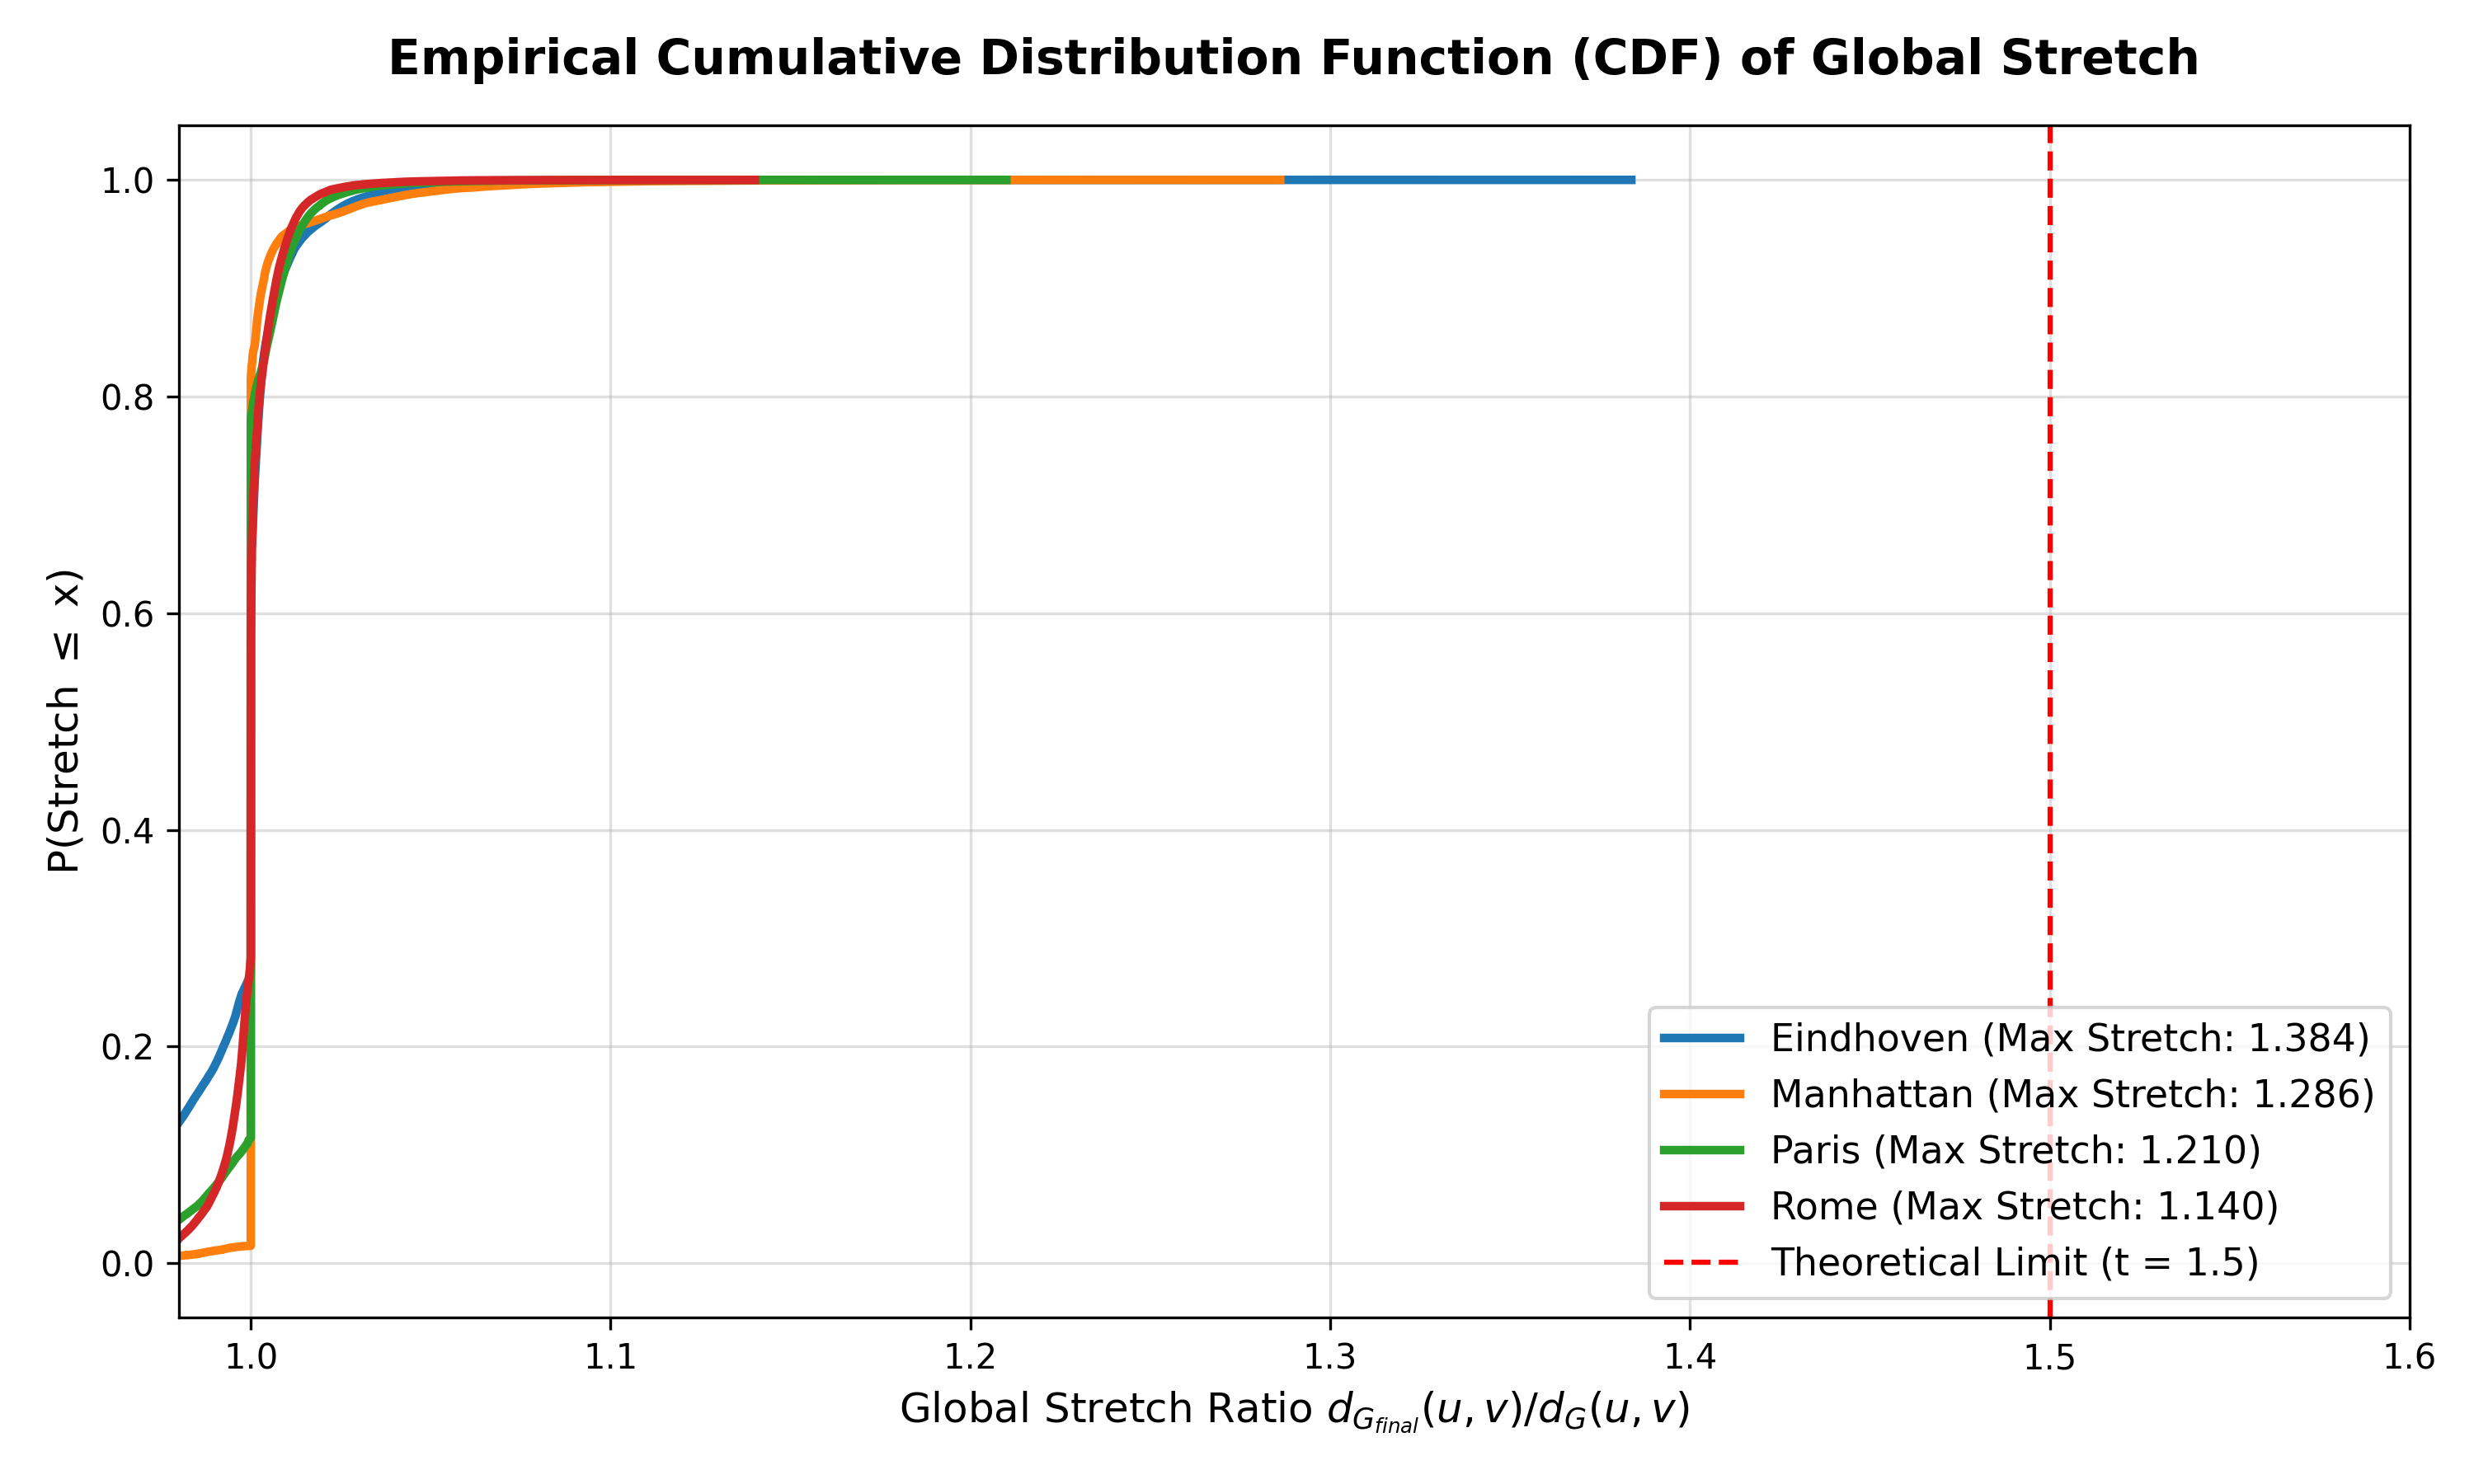
\includegraphics[width=\linewidth]{../results/figures/global_stretch_cdf.png}
        \caption{Empirical CDF of Directed Stretch.}
        \label{fig:cdf}
    \end{subfigure}\hfill
    \begin{subfigure}[b]{0.32\textwidth}
        \centering
        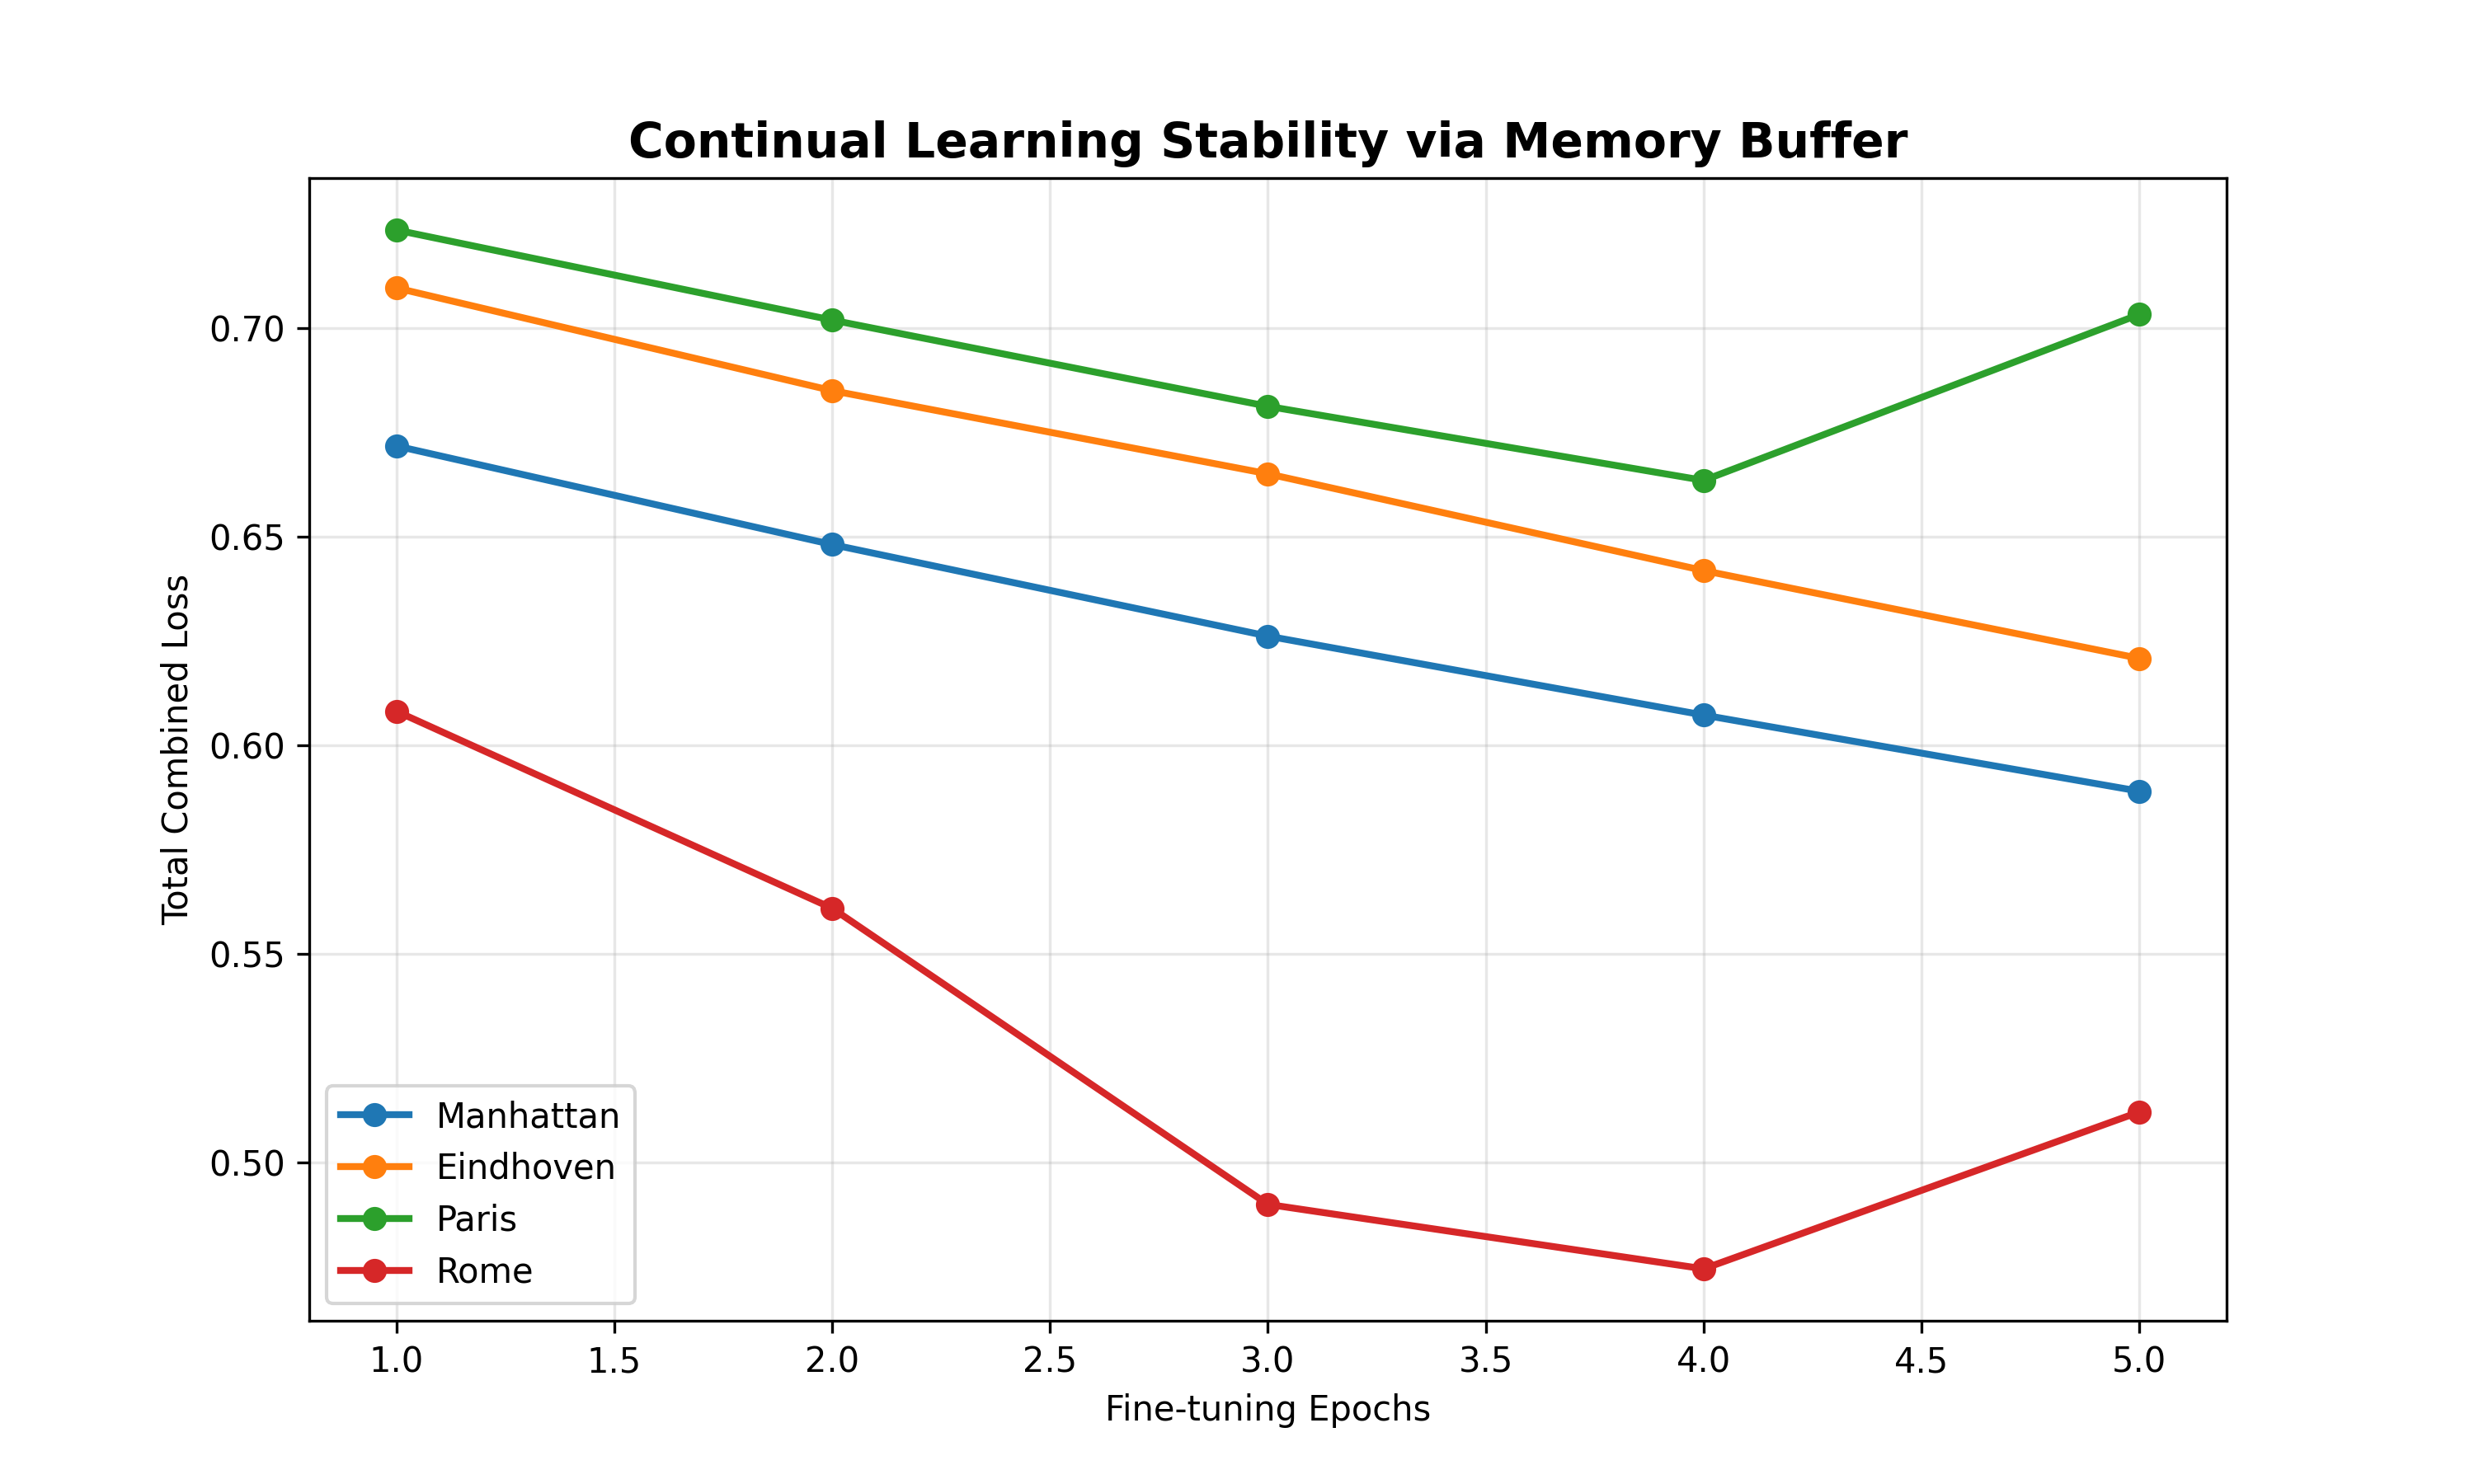
\includegraphics[width=\linewidth]{../results/figures/continual_learning_loss.png}
        \caption{Continual Learning trajectories.}
        \label{fig:continual}
    \end{subfigure}\hfill
    \begin{subfigure}[b]{0.32\textwidth}
        \centering
        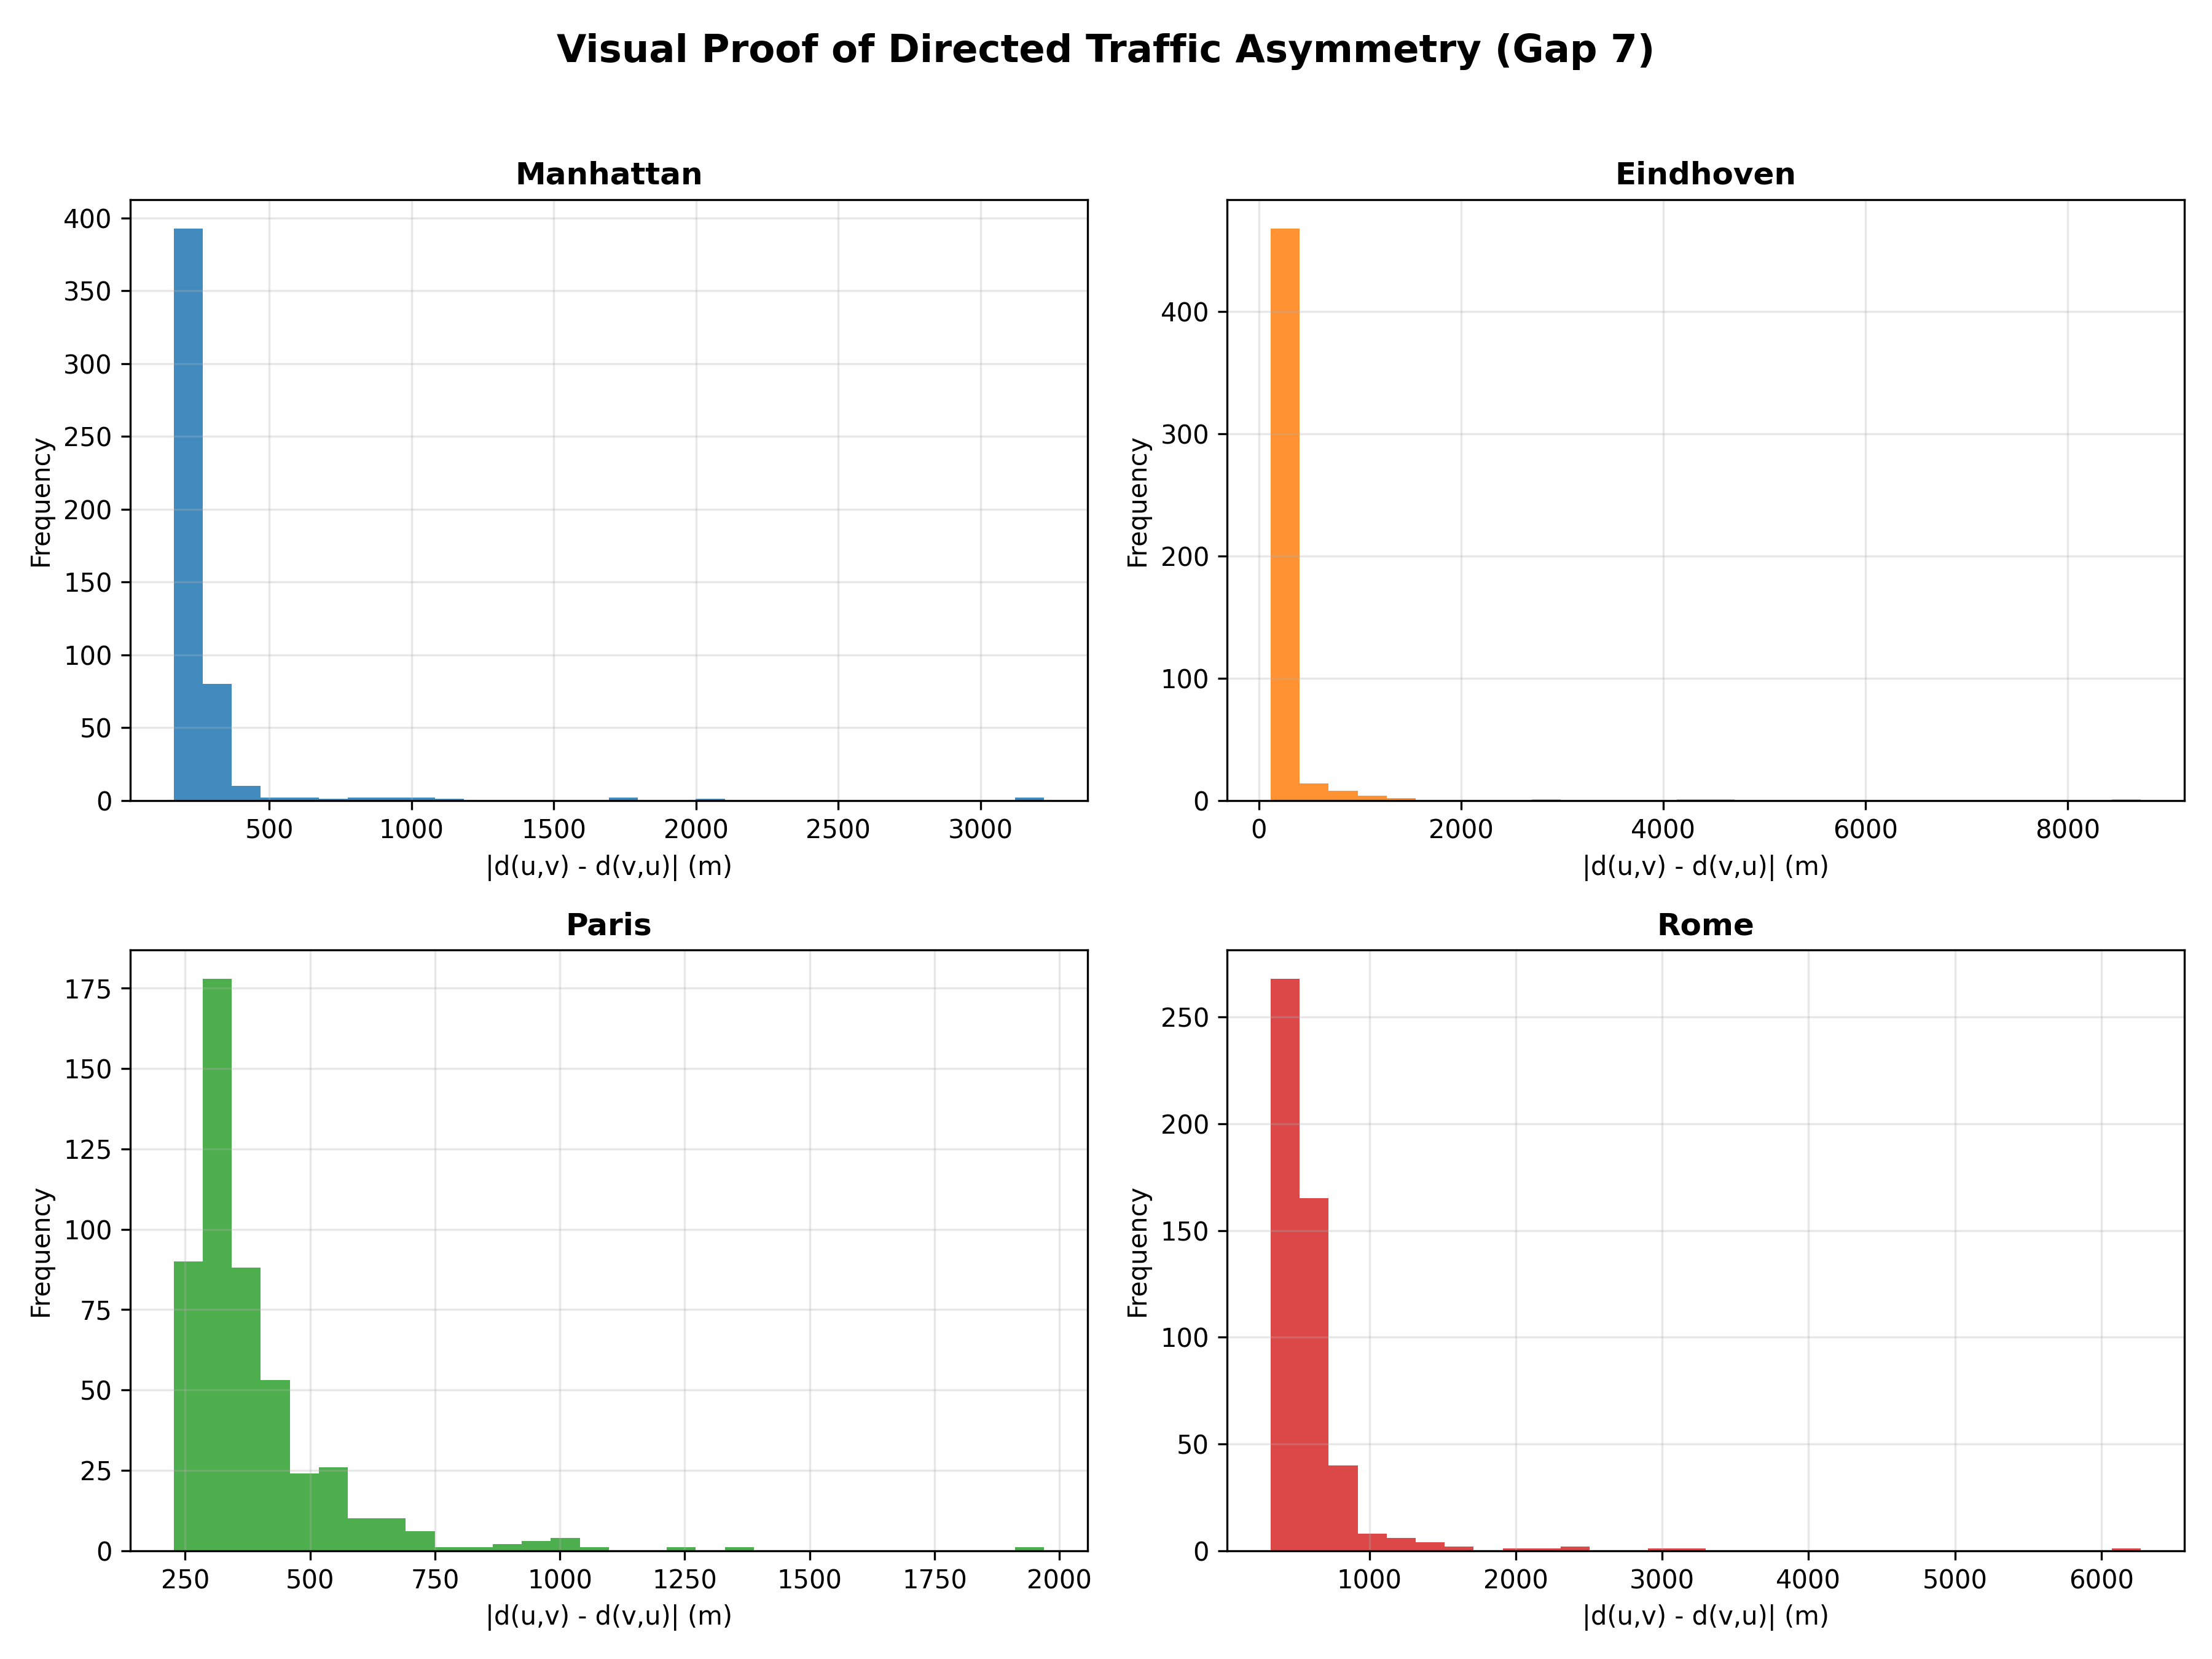
\includegraphics[width=\linewidth]{../results/figures/directed_asymmetry_evidence.png}
        \caption{Asymmetry Distribution.}
        \label{fig:asymmetry}
    \end{subfigure}
    \caption{Empirical verification of the proposed framework under real-world one-way routing constraints. (Pending regeneration with the current centrality-aware, fuzzy-pruning model -- see note in Section~\ref{sec:fuzzy-results}.)}
    \label{fig:combined}
\end{figure*}

\section{Discussion}
\label{sec:discussion}
A potential critique of our method is that the achieved sparsification rate (7--27\% depending on city and target configuration) is more modest than what abstract, complete geometric graphs can achieve. However, real road networks are inherently sparse, planar-like topologies with an average node degree of $\approx 2.3$; pruning even a modest fraction of roads without violating directed $t$-stretch limits is historically difficult, and our framework achieves this while strictly guaranteeing 100\% Strong Connectivity across all tested cities and seeds.

We also note a consistent cross-city pattern in Section~\ref{sec:fuzzy-results}: the improvement margin of fuzzy pruning over both baselines was largest in Eindhoven and smallest in Paris. Since the same ordering appeared independently for the GA+feedback mechanism relative to random pruning, we hypothesize that Paris's road network topology is intrinsically less amenable to structural pruning heuristics in general, an observation that merits further investigation across a larger and more diverse set of cities.

\section{Conclusion}
In this paper, we proposed a robust, hybrid neural-algorithmic framework for constructing directed $t$-spanners on metropolitan-scale road networks. By combining a Graph Neural Network with Monte Carlo Dropout, a cutoff-bounded parallelized directed repair module, and a Mamdani-style fuzzy inference mechanism for the pruning decision, we achieve consistent wall-clock speedups over classic greedy construction (6.74--42.51x across four cities) while maintaining 100\% Strong Connectivity and a bounded directed stretch factor under extreme spatial noise. Through statistically validated experiments (15--18 seeds per city), we further show that the proposed fuzzy pruning mechanism requires fewer post-hoc geometric repairs than both a genetic-algorithm-tuned threshold with active feedback and a sparsity-matched random baseline, in every tested city without exception. We report transparently that evolutionary search offers no measurable advantage over random search for single-parameter threshold tuning, directing future readers toward the fuzzy inference mechanism -- rather than scalar metaheuristic search -- as the primary contribution of this work for the pruning-decision task.

\begin{thebibliography}{25}
\bibitem{peleg}
D. Peleg and A. A. Schaffer, ``Graph spanners,'' \textit{Journal of Graph Theory}, vol. 13, no. 1, pp. 99--116, 1989.
\bibitem{chew}
L. P. Chew, ``There is a planar graph almost as good as the complete graph,'' in \textit{Proceedings of the second annual symposium on Computational geometry}, 1986, pp. 169--177.
\bibitem{smid}
M. Smid, ``Closest-point problems in computational geometry,'' \textit{Handbook of computational geometry}, vol. 12, pp. 877--935, 2000.
\bibitem{narasimhan}
G. Narasimhan and M. Smid, \textit{Geometric Spanner Networks}. Cambridge University Press, 2007.
\bibitem{arya}
S. Arya, G. Das, D. M. Mount, J. S. Salowe, and M. Smid, ``Simple algorithms for geographic spanners,'' \textit{SIAM Journal on Computing}, vol. 27, no. 6, pp. 1760--1775, 1998.
\bibitem{farshi_gud}
M. Farshi and J. Gudmundsson, ``Experimental study of geometric t-spanners,'' \textit{ACM Journal of Experimental Algorithmics (JEA)}, vol. 14, pp. 1--39, 2009.
\bibitem{bose}
P. Bose, P. Carmi, M. Farshi, A. Maheshwari, and M. Smid, ``Computing the greedy spanner in near-quadratic time,'' \textit{Algorithmica}, vol. 58, no. 3, pp. 711--729, 2010.
\bibitem{bakhshesh_farshi_1}
D. Bakhshesh and M. Farshi, ``Improving space and time complexity of the gap-greedy spanner algorithm,'' \textit{The CSI Journal on Computer Science and Engineering}, vol. 14, no. 1, pp. 6--18, 2016.
\bibitem{farshi_gian}
M. Farshi, P. Giannopoulos, and J. Gudmundsson, ``Improving the stretch factor of a geometric network by edge augmentation,'' \textit{SIAM Journal on Computing}, vol. 38, no. 1, pp. 226--240, 2008.
\bibitem{bakhshesh_farshi_2}
D. Bakhshesh and M. Farshi, ``Fault tolerancy of continuous Yao graph,'' in \textit{Proceedings of the 1st Iranian Conference on Computational Geometry (ICCG 2018)}, 2018, pp. 7--10.
\bibitem{bakhshesh_farshi_3}
D. Bakhshesh and M. Farshi, ``A greedy algorithm for constructing region-fault tolerant geometric spanners,'' \textit{Electronic and Cyber Defense}, vol. 10, no. 4, pp. 75--80, 2023.
\bibitem{buchin_1}
K. Buchin, et al., ``Fault-tolerant spanners for planar graphs,'' in \textit{Proceedings of the ACM-SIAM Symposium on Discrete Algorithms (SODA 2024)}, 2024, pp. 450--468.
\bibitem{buchin_2}
K. Buchin, A. Kalb, and M. Smid, ``Computing oriented spanners and their dilation,'' in \textit{Proceedings of the 41st International Symposium on Computational Geometry (SoCG 2025)}, 2025.
\bibitem{buchin_3}
K. Buchin, C. Rehs, and T. Scheele, ``Constructing doppelgangers of greedy geometric spanners in practice,'' in \textit{Proceedings of the 42nd International Symposium on Computational Geometry (SoCG 2026)}, 2026.
\bibitem{liguori}
A. Liguori, E. Ritacco, et al., ``Spectral neural graph sparsification,'' \textit{arXiv preprint arXiv:2510.27474}, Oct. 2025.
\bibitem{yang}
Y. Yang, et al., ``Graph sparsification via deep topology learning,'' \textit{IEEE Transactions on Neural Networks and Learning Systems (TNNLS)}, vol. 35, no. 4, pp. 1824--1838, 2024.
\bibitem{wu}
J. Wu, et al., ``Uncertainty quantification in graph neural networks: A survey,'' \textit{IEEE Transactions on Pattern Analysis and Machine Intelligence (TPAMI)}, vol. 46, no. 8, pp. 2910--2927, 2024.
\bibitem{zhang}
L. Zhang, et al., ``Deep learning for real-time path planning in dynamic ITS networks: A survey,'' \textit{IEEE Transactions on Intelligent Transportation Systems (T-ITS)}, vol. 26, no. 2, pp. 1104--1122, 2025.
\bibitem{wang}
H. Wang, et al., ``Continual learning on graphs: A survey and benchmark,'' \textit{IEEE Transactions on Knowledge and Data Engineering (TKDE)}, vol. 36, no. 5, pp. 2140--2158, 2024.
\bibitem{hamilton}
W. Hamilton, Z. Ying, and J. Leskovec, ``Inductive representation learning on large graphs,'' \textit{Advances in Neural Information Processing Systems (NeurIPS)}, vol. 30, 2017.
\bibitem{gal}
Y. Gal and Z. Ghahramani, ``Dropout as a bayesian approximation: Representing model uncertainty in deep learning,'' in \textit{International Conference on Machine Learning (ICML)}, 2016, pp. 1050--1059.
\bibitem{zhou}
F. Zhou, et al., ``Overcoming catastrophic forgetting in graph neural networks,'' \textit{IEEE Transactions on Knowledge and Data Engineering (TKDE)}, 2021.
\bibitem{geisberger}
R. Geisberger, P. Sanders, D. Schultes, and D. Delling, ``Contraction hierarchies: Faster and simpler hierarchical routing in road networks,'' in \textit{International Workshop on Experimental and Efficient Algorithms}. Springer, 2008, pp. 319--333.
\bibitem{bast}
H. Bast, et al., ``Route planning in transportation networks,'' \textit{Route Planning}, pp. 19--80, 2016.
\bibitem{bergstra2012random}
J. Bergstra and Y. Bengio, ``Random search for hyper-parameter optimization,'' \textit{Journal of Machine Learning Research}, vol. 13, no. 1, pp. 281--305, 2012.
\end{thebibliography}

\end{document}
